\documentclass[a4paper]{scrartcl}
\usepackage[utf8]{inputenc}			% Für Umlaute
\usepackage[T1]{fontenc}			% Für richtige Schrift
\usepackage[ngerman]{babel}			% Für neue deutsche Rechtschreibung (Trennung)
\usepackage{color}
\usepackage{amsmath}
\usepackage{amssymb}
\usepackage{graphicx}
\usepackage{textcomp}				% Fürs Gardzeichen

\usepackage{scrpage2}				% Für Kopf- und Fußzeilen
\pagestyle{scrheadings}				% Für Kopf- und Fußzeilen
\clearscrheadfoot					% Für Kopf- und Fußzeilen

\renewcommand{\labelenumi}{\alph{enumi})}
\renewcommand{\labelenumii}{\alph{enumii})}

\begin{document}
\titlehead{Wintersemester 2017/2018\\Motion Planning\\Prof. Horsch, Rudi Scheitler}
\author{David Welsch, Ken Hasenbank}
\title{Praktikum 2 - Potential Field Method}
\maketitle

\section*{Beschreibung der Aufgabe}

Das Ziel des Praktikums bestand darin, 3 Probleme mit Hilfe von Algorithmen der Potential-Field-Method zu lösen.
\\\\
Der Potential-Field-Method-Algorithmus vereint ein Potenzial in Richtung des Ziels (Attractive) mit einem Potenzial, welches von den Hindernissen weg zeigt (Repulsive) (siehe Abbildung \ref{img:Potential}). Sinn dieses Algorithmus ist es, dass der Roboter sich in Richtung des Ziels bewegt und von vorhandenen Hindernissen abgestoßen wird und somit nicht mit diesen kollidiert.\\ 
Ein Problem dieses Algorithmus besteht darin, dass es möglich ist, dass lokale Minima entstehen, bei denen der Roboter in einem solchen zum Stehen kommt und das Ziel nicht erreicht.\\
\begin{figure}[h!]
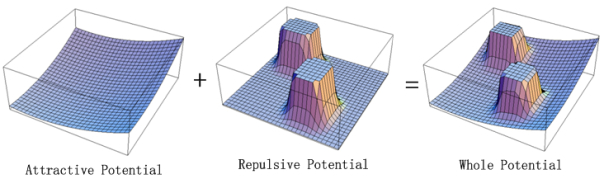
\includegraphics[width=\textwidth]{potential-field1_robot.jpg}
\caption{Potential Field Method}
\label{img:Potential}
\end{figure}

Eine Erweiterung der Potential-Field-Method stellt der Navigation-Function-Algorithmus dar. Dieser sorgt dafür, dass es im gesamten Raum nur ein Minimum gibt. Dieses Minimum ist bei korrekter Programmierung des Algorithmus und der richtigen Wahl des Parameters \textit{K} das Ziel. In Abbildung \ref{img:Potential2} ist dieser Algorithmus mit verschiedenen Parametern \textit{K} dargestellt.\\


\begin{figure}
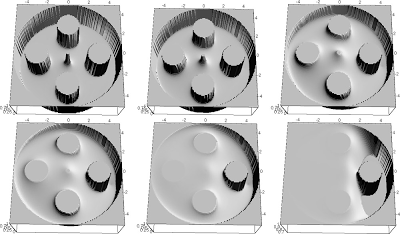
\includegraphics[width=\textwidth]{10_navigation_function_illustration.png}
\caption{Navigation Function}
\label{img:Potential2}
\end{figure}
Das Praktikum besteht aus drei Aufgaben. Diese unterscheiden sich folgendermaßen:
\begin{itemize}
\item Aufgabe 1\\ In der ersten Aufgabe ging es darum, den Potential-Field-Algorithmus zu implementieren.
\begin{enumerate}
\item 
In dieser Aufgabe waren die Objekte rechteckig.
\item 
In dieser Aufgabe waren die Objekte zylindrisch.
\end{enumerate}
\item Aufgabe 2 (Zusatzaufgabe)\\
In dieser Aufgabe sollte der Navigation Function Algorithmus implementiert werden. Die Objekte und Hindernisse waren dieselben wie in Aufgabe 1.b).

\end{itemize}



\section*{Beschreibung der L"osung}

Zur L"osung haben wir den vorgegeben Code-Rahmen verwendet. Wir haben die jeweiligen Funktionen in der Datei \textit{Potential.cpp} verwendet, um die jeweiligen Aufgaben zu lösen.
\begin{itemize}
\item Für Aufgabe 1.a) wurde die Funktion \textit{update\_box} genutzt. In dieser wird zuerst geschaut, ob das Ziel erreicht wurde (Zeile 118). Dies wird mit der Funktion \textit{goalReached} geprüft. Diese vergleicht die aktuelle Position mit der Zielposition und gibt beim unterschreiten eines Wertes, welcher durch die Konstante \textit{GOAL\_ERROR} beschrieben wird, \textit{true} zurück. Ist das Ziel erreicht, bricht die Funktion ab und gibt \textit{true} zurück.\\

Ansonsten wird zuerst der Vektor vom Roboter zum Ziel errechnet, dann die Distanz zum Ziel. Ist diese Distanz größer als eine festgelegte Mindestdistanz (\textit{DIST\_MIN\_GOAL}), wird der Vektor mit einem Skalierfaktor und der Mindestdistanz multipliziert, sowie durch die Länge geteilt. Dieser Vektor beschreibt dann das attraktive Potenzial, welches in Richtung des Ziels zeigt.\\

Anschließend wird das abweisende (repulsive) Potenzial berechnet. Hierzu wird zu jedem Objekt der Abstand zum Roboter berechnet, um zu sehen, ob das Objekt nah genug am Roboter ist, um den Roboter abzulenken. Dieser Abstand wird beschrieben durch die Konstante \textit{DIST\_MIN\_OBST}. Wenn ja, wird anhand der in der Aufgabenstellung gegebenen Formel $U_{rep,i}(q)$ berechnet.\\

Anschließend werden die beiden Potenziale addiert. Der daraus enstehende Vektor wird dann normalisiert und der Roboter in die durch den Vektor gegebene Richtung bewegt.\\

Damit ist die Aufgabe 1.a) abgeschlossen.

\item Die Aufgabe 1.b) wurde in der Funktion \textit{update\_cylinder} gelöst. Der Code entspricht genau dem der Aufgabe 1.a), lediglich die Variablen \textit{robot} sowie \textit{obstacle} sind nun Arrays der Klasse \textit{Cylinder} statt \textit{Box}. 

\item Die Aufgabe 2 (Zusatzaufgabe) wurde mit der Funktion \textit{update\_cylinder\_navigation} gelöst. Hier wird ebenfalls zuerst geprüft, ob das Ziel bereits erreicht wurde. Anschließend werden alle für die Berechnung der Ausrichtung benötigten Variablen berechnet. Diese sind in der Aufgabenstellung durch die Variable $\Delta$ $\gamma(q)$ beschrieben. Hierfür haben wir mehrere Unterfunktionen erstellt, welche im folgenden beschrieben werden:
\begin{itemize}
\item \textit{calc\_beta\_i}\\
In dieser Funktion wird die Variable $\beta_i(q)$ aus der Aufgabenstellung berechnet. Hierfür wird zuerst der Mittelpunkt des Roboters in der Variable \textit{pt} gespeichert. Ist \textit{i} größer als 0, wird anschließend von diesem Punkt der Mittelpunkt des zu betrachtenden Hindernisses abgezogen und die Länge berechnet. Zu dieser wird der Radius der beiden Objekte (Roboter und Hindernis) quadriert und von dem eben berechneten Wert abgezogen. Dies gilt nur, wenn $i > 0$ ist.\\
Ist $i==0$, so wird der zuerst berechnete Wert abgezogen und vom quadrierten Radius der beiden Objekte abgezogen.
\item \textit{calc\_beta}\\
In dieser Funktion wird die Variable $\beta(q)$ berechnet. Hierfür wird die eben beschriebene Funktion \textit{calc\_beta\_i} verwendet. Sie wird für jedes Objekt im Array der Hindernisse aufgerufen und zusammen multipliziert. Anschließend wird der Wert zurück gegeben.
\item \textit{calc\_p\_beta\_i}\\
In dieser Funktion wird der Vektor $\beta_i(q)$ aus der Aufgabenstellung berechnet. Dieser wird berechnet, indem die Mittelpunkte von Roboter und zu betrachtendem Objekt voneinander abgezogen und mit 2 multipliziert werden. Ist $i == 0$ wird der Vektor vor der Rückgabe noch negiert, um der Definition gerecht zu werden.
\item \textit{calc\_p\_beta}\\
In dieser Funktion wird der Vektor $\beta(q)$ aus der Aufgabenstellung berechnet. Hierfür werden die Funktionen \textit{calc\_p\_beta\_i} sowie \textit{calc\_beta\_i} verwendet. Diese werden entsprechend der Formel auf dem Aufgabenblatt aufsummiert bzw. multipliziert.
\end{itemize}
Außerdem wurden noch folgende Variablen berechnet:
\begin{itemize}
\item \textit{qminusgoal}\\
Hier wird der Vektor zwischen der aktuellen Konfiguration (dem Mittelpunkt des Roboters) sowie der Zielposition bestimmt. Der Vektor zeigt vom Roboter zum Ziel.
\item \textit{distgoal}\\
In dieser Variable wird die Länge des eben berechneten Vektors gespeichert.
\item \textit{beta}\\
In dieser Variable wird der Funktionswert von \textit{calc\_beta} gespeichert, damit die Funktion nur ein mal aufgerufen werden muss, obwohl der Wert in der endgültigen Berechnung mehrfach benötigt wird.
\item \textit{p\_beta}\\
Hier wird das Ergebnis von \textit{calc\_p\_beta} gespeichert, aus dem gleichen Grund wie oben.
\item \textit{distGoalBeta}\\
Hier wird die Variable \textit{disgoal} mit $2\times k$ potenziert und die Variable \textit{beta} hinzu addiert. Da dieser Wert bei unseren Berechnungen immer negativ wurde und er in der späteren Berechnung noch mit einer negativen Zahl potenziert werden muss, was zu einem undefinierten Ergebnis geführt hat, nehmen wir von dieser Zahl den Betrag.
\end{itemize}
Aus diesen Variablen kann dann der Vektor berechnet werden, der die Richtung der Bewegung des Roboters beschrieben soll. Unsere gesamte Formel dafür lautet:\\
$2 * qminusgoal\\
			* pow(distGoalBeta, 1 / k)\\
			- pow(distgoal, 2)  * (1 / k) * pow(distGoalBeta, (1 / k) - 1)\\
			* (2 * k * pow(distgoal, (2 * k) - 2) * qminusgoal + p_beta)\\
		) / (\\
			pow(distGoalBeta, 2 / k)$

In den verbleibenden Zeilen wird der Roboter dann in die eben berechnete Richtung fortbewegt und \textit{false} zurück gegeben, um der aufrufenden Funktion zu signalisieren, dass das Ziel noch nicht erreicht wurde.\\\\

Damit ist auch die Aufgabe 2 abgeschlossen.
\end{itemize}

\section*{Was wir gelernt haben}

Nachdem wir im ersten Praktikum bereits anschaulich gesehen haben, wie Wegfindungsalgorithmen aussehen können, war es nun sehr interessant für uns einen weiteren solchen Algorithmus zu implementieren und auch die Unterschiede zu sehen. Besonders die Zusatzaufgabe stellte dabei eine große Herausforderung dar, da die Formeln zum Teil schwer nachzuvollziehen waren.
\end{document}